
%%%%%%%%%%%%%%%%%%%%%%%%%%%%%%%%%%%%%%%%%%%%%%%%%%%%%%%%%%%%%%%%%%%%%%%%%%%%%%%%%%%%%%%
%%%%%%%%%%%%%%%%%%%%%%%%%%%%%%%%%%%%%%%%%%%%%%%%%%%%%%%%%%%%%%%%%%%%%%%%%%%%%%%%%%%%%%%
% 
% This top part of the document is called the 'preamble'.  Modify it with caution!
%
% The real document starts below where it says 'The main document starts here'.

\documentclass[12pt]{article}

\usepackage{amssymb,amsmath,amsthm}
\usepackage[top=1in, bottom=1in, left=1.25in, right=1.25in]{geometry}
\usepackage{fancyhdr}
\usepackage{enumerate}
\usepackage{listings}
\usepackage{graphicx}
\usepackage{float}
% Comment the following line to use TeX's default font of Computer Modern.

\usepackage{times,txfonts}



\makeatletter
\renewcommand*\env@matrix[1][*\c@MaxMatrixCols c]{%
  \hskip -\arraycolsep
  \let\@ifnextchar\new@ifnextchar
  \array{#1}}
\makeatother

\newtheoremstyle{homework}% name of the style to be used
  {18pt}% measure of space to leave above the theorem. E.g.: 3pt
  {12pt}% measure of space to leave below the theorem. E.g.: 3pt
  {}% name of font to use in the body of the theorem
  {}% measure of space to indent
  {\bfseries}% name of head font
  {:}% punctuation between head and body
  {2ex}% space after theorem head; " " = normal interword space
  {}% Manually specify head
\theoremstyle{homework} 

% Set up an Exercise environment and a Solution label.
\newtheorem*{exercisecore}{Exercise \@currentlabel}
\newenvironment{exercise}[1]
{\def\@currentlabel{#1}\exercisecore}
{\endexercisecore}

\newcommand{\localhead}[1]{\par\smallskip\noindent\textbf{#1}\nobreak\\}%
\newcommand\solution{\localhead{Solution:}}

%%%%%%%%%%%%%%%%%%%%%%%%%%%%%%%%%%%%%%%%%%%%%%%%%%%%%%%%%%%%%%%%%%%%%%%%
%
% Stuff for getting the name/document date/title across the header
\makeatletter
\RequirePackage{fancyhdr}
\pagestyle{fancy}
\fancyfoot[C]{\ifnum \value{page} > 1\relax\thepage\fi}
\fancyhead[L]{\ifx\@doclabel\@empty\else\@doclabel\fi}
\fancyhead[C]{\ifx\@docdate\@empty\else\@docdate\fi}
\fancyhead[R]{\ifx\@docauthor\@empty\else\@docauthor\fi}
\headheight 15pt

\def\doclabel#1{\gdef\@doclabel{#1}}
\doclabel{Use {\tt\textbackslash doclabel\{MY LABEL\}}.}
\def\docdate#1{\gdef\@docdate{#1}}
\docdate{Use {\tt\textbackslash docdate\{MY DATE\}}.}
\def\docauthor#1{\gdef\@docauthor{#1}}
\docauthor{Use {\tt\textbackslash docauthor\{MY NAME\}}.}
\makeatother

% Shortcuts for blackboard bold number sets (reals, integers, etc.)
\newcommand{\Reals}{\ensuremath{\mathbb R}}
\newcommand{\Nats}{\ensuremath{\mathbb N}}
\newcommand{\Ints}{\ensuremath{\mathbb Z}}
\newcommand{\Rats}{\ensuremath{\mathbb Q}}
\newcommand{\Cplx}{\ensuremath{\mathbb C}}
%% Some equivalents that some people may prefer.
\let\RR\Reals
\let\NN\Nats
\let\II\Ints
\let\CC\Cplx

%%%%%%%%%%%%%%%%%%%%%%%%%%%%%%%%%%%%%%%%%%%%%%%%%%%%%%%%%%%%%%%%%%%%%%%%%%%%%%%%%%%%%%%
%%%%%%%%%%%%%%%%%%%%%%%%%%%%%%%%%%%%%%%%%%%%%%%%%%%%%%%%%%%%%%%%%%%%%%%%%%%%%%%%%%%%%%%
% 
% The main document start here.

% The following commands set up the material that appears in the header.
\doclabel{STAT 402: Homework 9}
\docauthor{Stefano Fochesatto}
\docdate{\today}


%\textbf{Code:}
%\begin{center}
 %   \lstinputlisting{r1.txt}
%\end{center}

\begin{document}

\begin{exercise}{1} A common approach to estimating the total number of animals, 
  nests, etc. is to (1) fly or walk a transect (2) mark down each sighted object 
  (3)record characteristics such as experience of observer, weather, vegetation 
  type, size of object and especially distance from object to the transect(4) use a 
  model to assign detection probabilities to each object.\\
  \begin{enumerate}
    \item To estimate total number of animals, we will set $y_i = 1$ for all animals sighted. Why will this 
    an estimate of $N$, the number of animals?\\
    \solution This method allows us to take advantage of the detection probability. Suppose you knew the proportion of animals that 
    you could actually sample with your sampling scheme, that is the detection probability. Multiplying by the total number of possible animals 
    in a population will give you your expected sample size.\\
  \vspace{.15in}


  \item The chance that an animal is sighted is $\pi_i$, the Detection Probability. Note that the detection probability is the 
  chance of seeing the animal the one time we pass it. Why is this the inclusion probability only if we walk the transect exactly one time.?\\
  \solution Like we stated in the problem statement, the detection probability is the chance of seeing the animal the one time we pass it, the inclusion 
  probability is simply the probability that a sample is included in our experiment which is subject to change if we walk a transect more than once. 
  \vspace{.15in}
  
  \item We assume that sighting one animal does not change the chance of seeing another one, so that $\pi_{ij} = \pi_i\pi_j$. Can you think of a 
  situation where that would not be reasonable?\\
  \solution If the animal population exhibits herding behavior it's possible that a sighting of one animal could influence the probability of 
  sighting another. 
  \vspace{.15in}

  \item Why would the Hansen-Hurvits estimator be wrong,wrong, wrong for this data.\\
  \solution Hansen-Hurvits assumes we are taking multiply samples with replacement so there is no benefit to 
  making our sample larger. If we were walking multiple transects where the detection probability stayed the same between 
  transects it might be work. Also usually the probability used in the Hansen-Hurvets is related to sample/cluster size 
  and in this data it is connected to a detection function. 
  \vspace{.15in}
  
  
  \item Assume independent detection as in (c), use the Horvits-Thompson estimator(actually Hajek) to get an estimate of the 
  total number of animals and find its standard error. \\
  \solution  Like the questions suggests when we assume independent detection, the second term in the variance of the Horvits-Thompson 
  estimator goes to zero and we are left with just the Hajek estimator. Computing in r with the sample values set to 1 we get, an estimate of 
  29 animals with a CI of (52, 8).\\
  \textbf{Code:}
  \begin{center}
     \lstinputlisting{r1.txt}
  \end{center}
  
\end{enumerate}
\end{exercise}





\begin{exercise}{2} We fly a transect and ’sample’ a wolf track if it intersects out 
  flight path. The probability of sampling a track is the fraction of possible transect 
  that intersect the path ($\pi_i$) while $\pi_{ij}$ is the fraction of possible transects that 
  cross both paths. The transects are rows of the table below and each transect is 
  equally-likely to be selected as out path. The marked path is the one we actually 
  flew (so only consider paths that cross this). The number of wolves $y_i$ is at 
  the end of the path. Compute an estimator of the number of wolves and its standard 
  error. [ NOTE: In reality we would likely fly several independent transects, 
  compute the estimated total wolves (based on Horvitz-Thompson) for each one, 
  then treat the transects as units of a SRS and perform the simple SRS analysis.\\
  \solution First we need to compute the table of track sampling probabilities for the 
  tracks in our transect. Assume that the tracks are sampled left to right we get the following table. 
  \begin{equation*}
    \begin{bmatrix}
      Track & y_i & \pi_i & \pi_{ij}\\
      1 & 7 &  4/12 & 2/12, 1/12\\
      2 & 6 &  3/12 & 2/12, 2/12\\
      3 & 11 & 4/12 & 1/12, 2/12
    \end{bmatrix}
  \end{equation*}
  Computing the estimator and standard error in r we get a estimated total of 78 and a confidence interval of 
  (174, 24)\\
  \textbf{Code:}
  \begin{center}
     \lstinputlisting{r2.txt}
  \end{center}
  
\end{exercise}

\vspace{1in}




\begin{exercise}{3} We have divided a region into $N = 2000$ plots, each with area $.1$ Ha. 
  We only observed whether a fox has been in the area or not. From a SRS of size , we get the following 
  presence/absence data: absent in 8 of the 20 locations.\\
  \begin{enumerate}
    \item[a] We assume complete spacial randomness. What does this tell us about foxes?\\
    \solution Under the assumption of complete spatial randomness we know that the number of foxes in the $ith$ plot 
    will follow a poisson distribution with mean $\lambda(.1)$ where $\lambda$ is hectare density. With that in mind consider the probability 
    that a plot is empty, we get the following, 
    \begin{equation*}
      P(X = 0) = e^{-\lambda .1}
    \end{equation*}
    Note that from our SRS we have an estimate for the proportion of empty hectares, and therefore we can solve for $\hat{\lambda}$ with, 
    \begin{equation*}
      \hat{\lambda} = -\frac{1}{.1}ln(\frac{8}{20}) = 9.162907
    \end{equation*}
    Since there are $N = 1000$ plots we get that $\hat{\tau} = 9162.907$
  \end{enumerate}
  \vspace{.15in}

  \item[b.] Use the stocked quadrats method to get a 95 percent confidence interval fo the density of foxes.\\
  \solution Recall the stocked quadrats variance for $\lambda$, 
  \begin{equation*}
    V(\hat{\lambda})\approx \left(\dfrac{1}{na^2}\right)(e^{\lambda a} - 1) = \left(\dfrac{1}{20 .1^2}\right)(e^{9.162907 *.1} - 1)  = 7.5
  \end{equation*} 
  Therefore our 95 percent confidence interval comes out to, 
  \begin{equation*}
    95CI = \left(14.64013, 3.685681 \right)
  \end{equation*}
\end{exercise}

\vspace{1in}



\begin{exercise}{4} We want to estimate the number of ants in a large colony. 
  Each day we will capture 20 ants, count the number that are unmarked, 
  then mark all of them with a small colored dot. 
  We get the following data:\\
  Effort: 20, 20, 20, 20, 20, 20, 20, 20\\
  Catch (unmarked ants): 20, 18, 18, 16, 15, 15, 13, 15.\\
  \begin{enumerate}
    \item[a.] Compute CPUE and CC at each time period. Plot them against each other. Does CPUE seem to decrease over time?\\
    \solution From the plot it does seem as though CPUE is dropping as we continue to catch more of the population. It helps that the 
    effort is staying constant and we can attribute this relationship to the change in population size. Plotting in r we get,  
    \begin{figure}[H]
      \begin{center}
        \caption(CPUE vs CC)
      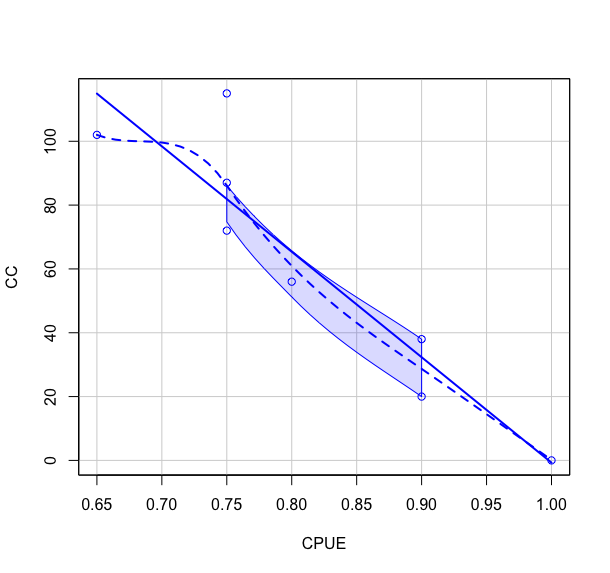
\includegraphics[width = .9\textwidth]{Rplot.png}
      \end{center}
    \end{figure}
    \textbf{Code:}
    \begin{center}
       \lstinputlisting{r3.txt}
    \end{center}
    \vspace{.15in}


    \item[b.] Get a 95 percent confidence interval for the total number of ants.\\
    \solution \textbf{Code:}
    \begin{center}
       \lstinputlisting{r3.txt}
    \end{center}

  \end{enumerate}
  
\end{exercise}







\end{document}




















